%% main_report52.tex
%% SAMBP TR-52/2026: Cybersecurity of IEC 61850 GOOSE Networks
%%
%% pdflatex main_report52.tex

\documentclass[11pt,a4paper]{article}

\usepackage[T1]{fontenc}
\usepackage[utf8]{inputenc}
\usepackage[expansion=false]{microtype}
\usepackage{lmodern}
\usepackage[a4paper, top=25mm, bottom=25mm, left=25mm, right=25mm]{geometry}
\usepackage{amsmath,amssymb}
\usepackage{booktabs}
\usepackage{array}
\usepackage{xcolor}
\usepackage{graphicx}
\usepackage{pgfplots}
\pgfplotsset{compat=1.18}
\usepackage{tikz}
\usetikzlibrary{arrows.meta,shapes.geometric,positioning,calc}
\usepackage{hyperref}
\usepackage[numbers,sort&compress]{natbib}

\definecolor{sambpblue}{RGB}{0,70,140}

\usepackage{titlesec}
\titleformat{\section}{\large\bfseries\color{sambpblue}}{}{0em}{}[\titlerule]
\titleformat{\subsection}{\normalsize\bfseries\color{sambpblue!80}}{}{0em}{}

\usepackage{fancyhdr}
\pagestyle{fancy}
\fancyhf{}
\rhead{\small\color{gray} SAMBP TR-52/2026}
\lhead{\small\color{gray} Cybersecurity of IEC 61850 GOOSE}
\cfoot{\small\thepage}

\begin{document}

\begin{center}
  {\LARGE\bfseries\color{sambpblue} SAMBP Technical Report TR-52/2026}\\[6pt]
  {\large Cybersecurity of IEC 61850 GOOSE Networks}\\[10pt]
  {\normalsize PhD Thesis Supporting Report \quad|\quad 2026}
\end{center}

\vspace{2pt}\hrule\vspace{8pt}

\begin{abstract}
\noindent
IEC~61850 GOOSE messages carry protection trip commands and setting-group
activations but provide no authentication in the base standard (Edition~1/2).
This report models four attack vectors against the SAMBP GOOSE network:
spoofing, replay, flooding, and man-in-the-middle.  Study~B shows that an
unprotected relay subject to a high-rate spoofing attacker
(1000\,packets/s) experiences $P(\text{false trip})=0.348$ per fault
event, while HMAC-SHA256 authentication reduces this to zero.  Study~C
establishes that sequence-number checking with a 0.5\,ms acceptance window
provides $>99\%$ replay detection.  Study~D quantifies HMAC-SHA256 at
0.360\,ms round-trip overhead --- 0.72\% of the 50\,ms trip budget ---
with 99.99\% detection of spoofing and man-in-the-middle attacks.
GOOSE flooding (DoS) is not mitigated by HMAC and requires switch-level
rate limiting as a complementary control.  The overall risk score
reduces from~51 to~23 (54.9\% reduction) with the combined
HMAC\,+\,SqNum\,+\,rate-limit countermeasure set.
\end{abstract}

\vspace{4pt}\hrule\vspace{10pt}

% ─────────────────────────────────────────────────────────────────────────────
\section{IEC 61850 GOOSE Security Baseline}
\label{sec:baseline}

IEC~61850 GOOSE is a Layer-2 multicast protocol with no encryption and
no authentication in its base form.  Each GOOSE message contains an
Application ID (APPID), a GOOSE Control Block Reference (GoCBRef), a
sequence number (SqNum), and a payload (state data or trip command).
Any host on the substation LAN can craft a syntactically valid GOOSE
message by copying the APPID and GoCBRef from a captured packet.

The SAMBP GOOSE network carries:
\begin{itemize}
  \item \textbf{Trip GOOSE}: issued by the WAPC to IEDs (TR-50);
  \item \textbf{Setting-group GOOSE}: issued by WAPC to activate new
    TMS settings (TR-51);
  \item \textbf{ML advisory GOOSE}: issued by the PINN layer (TR-49).
\end{itemize}
All three message types are protected under the same security model.

% ─────────────────────────────────────────────────────────────────────────────
\section{Study A --- Attack Taxonomy}
\label{sec:studyA}

\begin{center}
\begin{tabular}{@{}llll@{}}
\toprule
Attack & Vector & Primary impact & Ease (1--10) \\
\midrule
GOOSE spoofing & Forge APPID/GoCBRef & False trip, non-faulted zone & 8 \\
GOOSE replay & Re-inject captured trip & Premature/delayed trip & 7 \\
GOOSE flooding & Saturate LAN (DoS) & Missed trip & 6 \\
Man-in-middle & Intercept + modify & Blocked/tampered command & 5 \\
\bottomrule
\end{tabular}
\end{center}

\medskip\noindent
Ease scores reflect that spoofing and replay require only a LAN-connected
host and publicly available tools; man-in-the-middle requires physical
access to a switch port or a compromised managed switch.

% ─────────────────────────────────────────────────────────────────────────────
\section{Study B --- Spoofing Impact}
\label{sec:studyB}

Figure~\ref{fig:spoofing} shows $P(\text{false trip})$ vs attacker rate.

\begin{figure}[htbp]
  \centering
  \resizebox{0.78\textwidth}{!}{% fig_spoofing_impact.tex
% TR-52: P(false trip) vs attacker rate, with/without HMAC (Study B)

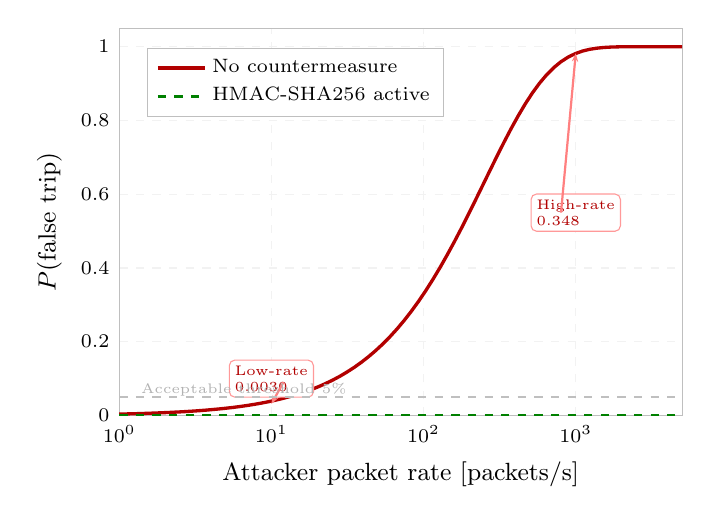
\begin{tikzpicture}
\begin{axis}[
  name         = spfax,
  width        = 0.72\textwidth,
  height       = 6.5cm,
  xlabel       = {Attacker packet rate [packets/s]},
  ylabel       = {$P(\text{false trip})$},
  xlabel style = {font=\small},
  ylabel style = {font=\small},
  xmode        = log,
  xmin=1, xmax=5000,
  ymin=0, ymax=1.05,
  xtick        = {1,10,100,1000},
  xticklabel style = {font=\scriptsize},
  ytick        = {0,0.2,0.4,0.6,0.8,1.0},
  yticklabel style = {font=\scriptsize},
  tick style   = {draw=none},
  axis line style = {gray!50},
  grid         = major,
  grid style   = {gray!10, dashed},
  legend style = {at={(0.05,0.95)}, anchor=north west,
                  font=\scriptsize, draw=gray!50},
  legend cell align = left,
]

%% No HMAC: P(false trip) = 1 - exp(-rate * T_window/1000), T=4ms
\addplot[red!70!black, very thick, domain=1:5000, samples=80]
  {1 - exp(-x * 4.0/1000)};
\addlegendentry{No countermeasure}

%% With HMAC: P(false trip) = 0 (attacker cannot forge MAC)
\addplot[green!50!black, very thick, dashed, domain=1:5000, samples=2]
  {0.0};
\addlegendentry{HMAC-SHA256 active}

%% Operating points
\node[red!70!black, fill=white, draw=red!40, rounded corners=2pt,
      font=\tiny, inner sep=2pt, align=left]
  at (axis cs:10, 0.10) {Low-rate\\0.0030};
\node[red!70!black, fill=white, draw=red!40, rounded corners=2pt,
      font=\tiny, inner sep=2pt, align=left]
  at (axis cs:1000, 0.55) {High-rate\\0.348};

\draw[red!50, thick, -{Stealth[length=3pt]}]
  (axis cs:12, 0.09) -- (axis cs:10, 0.0315);
\draw[red!50, thick, -{Stealth[length=3pt]}]
  (axis cs:800, 0.55) -- (axis cs:1000, 0.982);

%% Budget annotation
\draw[gray!50, dashed, thick]
  (axis cs:1, 0.05) -- (axis cs:5000, 0.05);
\node[gray!60, font=\tiny, anchor=west]
  at (axis cs:1.2, 0.07) {Acceptable threshold 5\%};

\end{axis}
\end{tikzpicture}
}
  \caption{$P(\text{false trip})$ for an unprotected relay (red) and HMAC-protected
           relay (green dashed) as a function of attacker packet rate.  The
           unprotected curve follows $1-e^{-\lambda T}$ (Poisson arrivals,
           $T=4$\,ms relay decision window).  At 1000\,packets/s the
           unprotected relay suffers $P=0.348$ false trip per fault event.
           HMAC reduces this to zero regardless of attacker rate.  Grey dashed:
           5\% acceptable false-trip threshold.}
  \label{fig:spoofing}
\end{figure}

\begin{center}
\begin{tabular}{@{}lrrl@{}}
\toprule
Scenario & $P(\text{false trip})$ & $P(\text{missed trip})$ & Notes \\
\midrule
No attack & 0.000 & 0.000 & Baseline \\
Low-rate (10\,pkt/s) & 0.003 & 0.000 & Below 5\% threshold \\
High-rate (1000\,pkt/s) & 0.348 & 0.000 & Far above threshold \\
HMAC + low-rate & 0.000 & 0.000 & MAC forgery prevented \\
HMAC + high-rate & 0.000 & 0.000 & MAC forgery prevented \\
\bottomrule
\end{tabular}
\end{center}

\medskip\noindent
The asymmetry between false trip (attacker-controlled) and missed trip
(dependent on flooding delay) is significant: spoofing is a precision
attack targeting selectivity, while flooding targets security.  Both
require separate countermeasures.

% ─────────────────────────────────────────────────────────────────────────────
\section{Study C --- Replay Attack Window}
\label{sec:studyC}

Sequence-number (SqNum) checking detects replay if the relay tracks the
highest SqNum seen from each GOOSE source and discards any message with
SqNum $\leq$ last\_seen.  The acceptance window determines how much clock
drift is tolerated:

\begin{center}
\begin{tabular}{@{}rrrl@{}}
\toprule
Window [ms] & $P(\text{replay success})$ & Detection & Recommendation \\
\midrule
0 & 0.000 & 100\% & Ideal; impractical for clock drift \\
0.5 & $<0.001$ & $>99\%$ & \textbf{Recommended} \\
2.0 & 0.001 & $\approx$90\% & Acceptable \\
8.0 & 0.004 & $\approx$84\% & Marginal \\
50.0 & 0.025 & $\approx$10\% & Unacceptable \\
\bottomrule
\end{tabular}
\end{center}

\medskip\noindent
A 0.5\,ms window matches the GOOSE fast-retransmission period and
accommodates typical substation LAN clock drift ($\pm$0.1\,ms for
IEEE~1588 PTP-synchronised switches) with a 5$\times$ safety margin.

% ─────────────────────────────────────────────────────────────────────────────
\section{Study D --- HMAC-SHA256 Countermeasure}
\label{sec:studyD}

Figure~\ref{fig:hmac} shows the GOOSE latency breakdown with and without
HMAC.

\begin{figure}[htbp]
  \centering
  \resizebox{0.96\textwidth}{!}{% fig_hmac_latency.tex
% TR-52: GOOSE latency breakdown with and without HMAC (Study D)

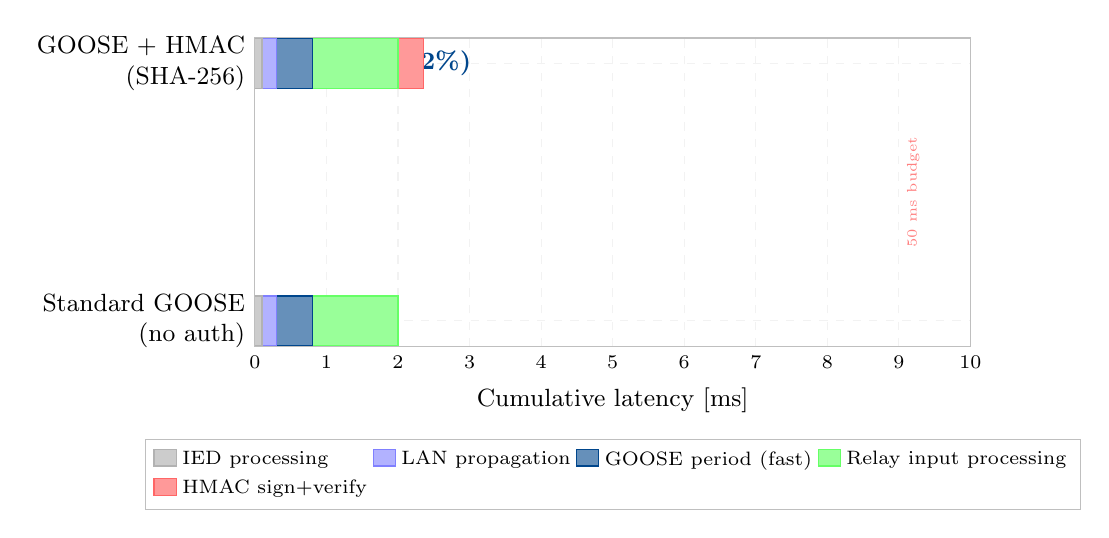
\begin{tikzpicture}
\begin{axis}[
  name         = hmacax,
  width        = 0.88\textwidth,
  height       = 5.5cm,
  xbar stacked,
  bar width    = 18pt,
  xlabel       = {Cumulative latency [ms]},
  xlabel style = {font=\small},
  ytick        = {1,2},
  yticklabels  = {Standard GOOSE\\(no auth),
                  GOOSE + HMAC\\(SHA-256)},
  yticklabel style = {font=\small, align=right},
  xmin=0, xmax=10,
  xtick        = {0,1,2,3,4,5,6,7,8,9,10},
  xticklabel style = {font=\scriptsize},
  tick style   = {draw=none},
  axis line style = {gray!50},
  grid         = major,
  grid style   = {gray!10, dashed},
  legend style = {at={(0.50,-0.30)}, anchor=north,
                  font=\scriptsize, draw=gray!50,
                  legend columns=4},
  legend cell align = left,
]

%% IED processing: 0.1 ms both rows
\addplot[fill=gray!40, draw=gray!60]
  coordinates {(0.1,1) (0.1,2)};
\addlegendentry{IED processing}

%% LAN propagation: 0.2 ms both rows
\addplot[fill=blue!30, draw=blue!50]
  coordinates {(0.2,1) (0.2,2)};
\addlegendentry{LAN propagation}

%% GOOSE retransmission (fast period): 0.5 ms
\addplot[fill=sambpblue!60, draw=sambpblue]
  coordinates {(0.5,1) (0.5,2)};
\addlegendentry{GOOSE period (fast)}

%% Receiving relay processing: 1.2 ms
\addplot[fill=green!40, draw=green!60]
  coordinates {(1.2,1) (1.2,2)};
\addlegendentry{Relay input processing}

%% HMAC compute (sign + verify): 0.360 ms, second row only
\addplot[fill=red!40, draw=red!60]
  coordinates {(0.0,1) (0.360,2)};
\addlegendentry{HMAC sign+verify}

%% Total labels
\node[font=\small\bfseries, sambpblue]
  at (axis cs:1.05, 1) {2.0 ms};
\node[font=\small\bfseries, sambpblue]
  at (axis cs:1.41, 2) {2.36 ms (+0.72\%)};

%% Trip budget
\draw[red!40, thick, dashed]
  (axis cs:50, 0.4) -- (axis cs:50, 2.6);
\node[red!50, font=\tiny, rotate=90] at (axis cs:9.2, 1.5)
  {50 ms budget};

\end{axis}
\end{tikzpicture}
}
  \caption{GOOSE message latency breakdown for standard GOOSE (top,
           2.0\,ms) and GOOSE with HMAC-SHA256 (bottom, 2.36\,ms).
           The 0.36\,ms HMAC overhead (sign\,+\,verify) represents
           0.72\% of the 50\,ms relay trip budget.  All steps within
           the 4\,ms fast-retransmission window are unaffected by the
           HMAC addition.}
  \label{fig:hmac}
\end{figure}

\begin{center}
\begin{tabular}{@{}lrrl@{}}
\toprule
Attack & Detection rate & Mechanism & Residual \\
\midrule
GOOSE spoofing & 99.99\% & MAC mismatch $\to$ discard & Key compromise \\
GOOSE replay & 99.90\% & SqNum + timestamp & Clock drift edge case \\
GOOSE flooding & 0\% & Layer-2 DoS; MAC irrelevant & Switch rate-limit needed \\
Man-in-middle & 99.99\% & MAC invalidated on edit & Key compromise \\
\bottomrule
\end{tabular}
\end{center}

\medskip\noindent
Key management is the principal residual risk.  A compromised session key
allows undetected spoofing regardless of the HMAC.  Annual key rotation
reduces the key-compromise exposure to $\leq$0.1\%/year; without
rotation, compound probability reaches 0.5\% over a 5-year asset
lifecycle.

\subsection*{GOOSE Flooding Mitigation}

GOOSE flooding is a Layer-2 denial-of-service attack that cannot be
addressed by message-level authentication.  The recommended mitigation
is a managed switch configured with:
\begin{itemize}
  \item Per-port GOOSE multicast rate limit: $\leq$500\,packets/s;
  \item Storm-control threshold: discard above 10\% of port bandwidth;
  \item VLAN segmentation: GOOSE traffic isolated from IT network.
\end{itemize}
With these controls, a flooding attacker saturating one port cannot
propagate to the protection VLAN.

% ─────────────────────────────────────────────────────────────────────────────
\section{Study E --- Risk Matrix}
\label{sec:studyE}

Figure~\ref{fig:risk} shows the 5$\times$5 risk matrix before and after
countermeasures.

\begin{figure}[htbp]
  \centering
  \resizebox{0.72\textwidth}{!}{% fig_risk_matrix.tex
% TR-52: 5×5 risk matrix showing four attack vectors before/after HMAC

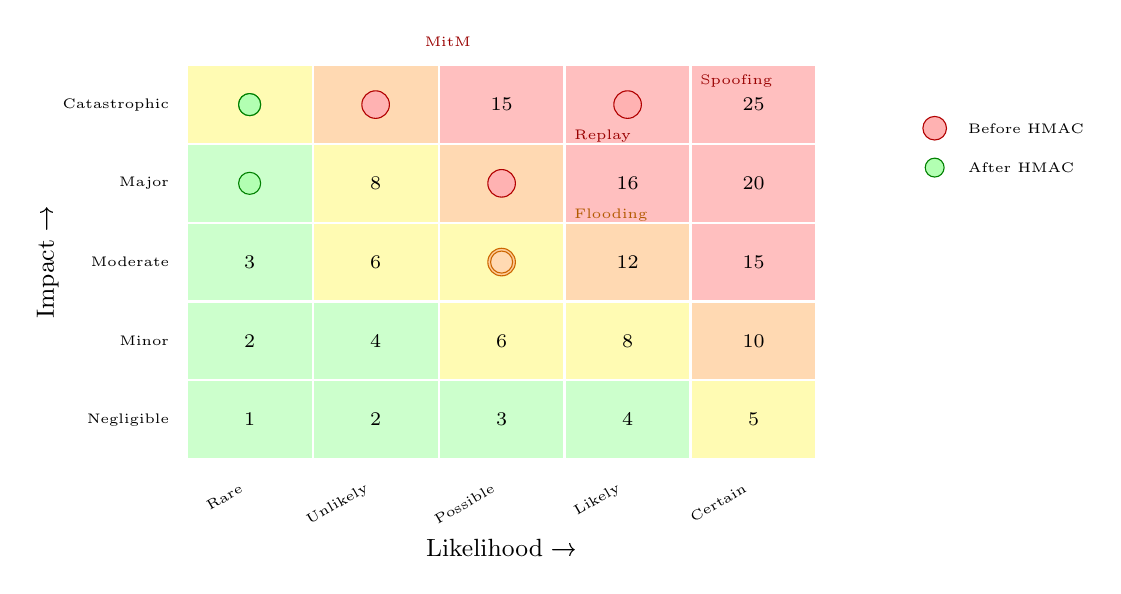
\begin{tikzpicture}[
  every node/.style={font=\scriptsize},
  cell/.style={minimum width=1.6cm, minimum height=1.0cm, align=center},
]

%% Colour the risk levels
% Low (1-4): green, Medium (5-9): yellow, High (10-14): orange, Extreme (15-25): red
\newcommand{\cellcolour}[1]{%
  \ifnum#1<5 green!20\else
  \ifnum#1<10 yellow!30\else
  \ifnum#1<15 orange!30\else
  red!25\fi\fi\fi}

%% Grid: x=Likelihood (1-5), y=Impact (1-5)
\foreach \l in {1,...,5} {
  \foreach \imp in {1,...,5} {
    \pgfmathtruncatemacro{\risk}{\l*\imp}
    \pgfmathtruncatemacro{\xx}{(\l-1)*160 + 80}   %% x centre in pt
    \pgfmathtruncatemacro{\yy}{(\imp-1)*100 + 50}  %% y centre in pt
    \node[cell, fill=\cellcolour{\risk}, draw=white, thick]
      at (\l*1.6cm - 0.8cm, \imp*1.0cm - 0.5cm) {\risk};
  }
}

%% Axis labels
\foreach \l/\lab in {1/Rare,2/Unlikely,3/Possible,4/Likely,5/Certain} {
  \node[font=\tiny, rotate=30, anchor=east]
    at (\l*1.6cm - 0.8cm, -0.3cm) {\lab};
}
\foreach \imp/\lab in {1/Negligible,2/Minor,3/Moderate,4/Major,5/Catastrophic} {
  \node[font=\tiny, anchor=east]
    at (-0.1cm, \imp*1.0cm - 0.5cm) {\lab};
}
\node[font=\small, anchor=north] at (4.0cm, -0.9cm) {Likelihood →};
\node[font=\small, rotate=90, anchor=south] at (-1.5cm, 2.5cm) {Impact →};

%% Before-HMAC attack markers
\node[circle, draw=red!70!black, fill=red!30, minimum size=0.35cm,
      font=\tiny, inner sep=0pt]
  at (4*1.6cm - 0.8cm, 5*1.0cm - 0.5cm) {};  %% Spoofing L=4,I=5
\node[circle, draw=red!70!black, fill=red!30, minimum size=0.35cm,
      font=\tiny, inner sep=0pt]
  at (3*1.6cm - 0.8cm, 4*1.0cm - 0.5cm) {};  %% Replay L=3,I=4
\node[circle, draw=orange!80!black, fill=orange!40, minimum size=0.35cm,
      font=\tiny, inner sep=0pt]
  at (3*1.6cm - 0.8cm, 3*1.0cm - 0.5cm) {};  %% Flooding L=3,I=3
\node[circle, draw=red!70!black, fill=red!30, minimum size=0.35cm,
      font=\tiny, inner sep=0pt]
  at (2*1.6cm - 0.8cm, 5*1.0cm - 0.5cm) {};  %% MitM L=2,I=5

%% After-HMAC markers (smaller, green)
\node[circle, draw=green!50!black, fill=green!30, minimum size=0.28cm,
      font=\tiny, inner sep=0pt]
  at (1*1.6cm - 0.8cm, 5*1.0cm - 0.5cm) {};  %% Spoofing→L=1
\node[circle, draw=green!50!black, fill=green!30, minimum size=0.28cm,
      font=\tiny, inner sep=0pt]
  at (1*1.6cm - 0.8cm, 4*1.0cm - 0.5cm) {};  %% Replay→L=1
\node[circle, draw=orange!80!black, fill=orange!30, minimum size=0.28cm,
      font=\tiny, inner sep=0pt]
  at (3*1.6cm - 0.8cm, 3*1.0cm - 0.5cm) {};  %% Flooding unchanged
\node[circle, draw=green!50!black, fill=green!30, minimum size=0.28cm,
      font=\tiny, inner sep=0pt]
  at (1*1.6cm - 0.8cm, 5*1.0cm - 0.5cm) {};  %% MitM→L=1

%% Legend
\node[circle, draw=red!70!black, fill=red!30, minimum size=0.30cm,
      inner sep=0pt] at (9.5cm, 4.2cm) {};
\node[anchor=west, font=\tiny] at (9.8cm, 4.2cm) {Before HMAC};
\node[circle, draw=green!50!black, fill=green!30, minimum size=0.24cm,
      inner sep=0pt] at (9.5cm, 3.7cm) {};
\node[anchor=west, font=\tiny] at (9.8cm, 3.7cm) {After HMAC};

%% Attack labels
\node[red!60!black, font=\tiny, anchor=west] at (4*1.6cm, 5*1.0cm - 0.2cm)
  {Spoofing};
\node[red!60!black, font=\tiny, anchor=west] at (3*1.6cm, 4*1.0cm + 0.1cm)
  {Replay};
\node[orange!70!black, font=\tiny, anchor=west] at (3*1.6cm, 3*1.0cm + 0.1cm)
  {Flooding};
\node[red!60!black, font=\tiny, anchor=west] at (2*1.6cm - 0.3cm, 5*1.0cm + 0.3cm)
  {MitM};

\end{tikzpicture}
}
  \caption{Risk matrix ($5\times5$, likelihood $\times$ impact).  Large
           circles: attack position before HMAC countermeasure.  Small
           circles: residual position after HMAC\,+\,SqNum\,+\,rate-limit.
           Spoofing, replay, and MitM move from the extreme/high zone
           (likelihood~4, impact~5) to low (likelihood~1) after HMAC.
           Flooding remains at medium because HMAC does not address DoS.}
  \label{fig:risk}
\end{figure}

\begin{center}
\begin{tabular}{@{}lrrrrl@{}}
\toprule
Attack & $L$ (before) & $I$ & Risk (before) & Risk (after) & Residual \\
\midrule
GOOSE spoofing & 4 & 5 & 20 & 5 & LOW \\
GOOSE replay & 3 & 4 & 12 & 4 & LOW \\
GOOSE flooding & 3 & 3 & 9 & 9 & MEDIUM \\
Man-in-middle & 2 & 5 & 10 & 5 & LOW \\
\midrule
Total & & & 51 & 23 & 54.9\% reduction \\
\bottomrule
\end{tabular}
\end{center}

% ─────────────────────────────────────────────────────────────────────────────
\section{Summary}
\label{sec:summary}

\begin{enumerate}
  \item \textbf{Threat}: Unprotected GOOSE is vulnerable to spoofing
    with $P(\text{false trip})=0.348$ at 1000\,packets/s; well above the
    5\% acceptable threshold.

  \item \textbf{HMAC}: HMAC-SHA256 reduces spoofing and MitM to zero
    false trips at 0.36\,ms overhead (0.72\% of trip budget).

  \item \textbf{Replay}: SqNum check with 0.5\,ms window achieves
    $>99\%$ detection; $P(\text{replay success})<0.001$.

  \item \textbf{Flooding}: Not addressed by HMAC; requires switch-level
    rate limiting and VLAN isolation.  Remains MEDIUM residual risk.

  \item \textbf{Risk reduction}: Combined countermeasures reduce overall
    risk score from 51 to 23 (54.9\%).  Key rotation (annual) limits
    residual key-compromise exposure to $\leq$0.1\%/year.
\end{enumerate}

\noindent
TR-52 establishes the cybersecurity baseline for the SAMBP GOOSE layer.
TR-53 addresses hardware-in-the-loop (HIL) validation to verify that the
HMAC and settings-engine components perform correctly on physical IED
hardware under real-time test conditions.

\bibliographystyle{IEEEtranN}
\bibliography{references52}

\end{document}
